% !TEX root = ../Диплом.tex

\section{Эксперименты}

Сравним число шагов, которые понадобятся ID-DLS с разным выбором эвристик, чтобы квадратизировать различные нелинейные системы.



\begin{table}[h!]
\centering
\resizebox{\textwidth}{!}{
\begin{tabular}{||c c c c c c c||} 
     \hline
     Nonlinear system & Random & FF & FVC & AED & AEQD & SMD \\ [0.5ex] 
     \hline\hline
     xSigmoid & 145$\pm$ 85 & 140 $\pm$ 83 & 273 $\pm$ 4 & 146 $\pm$ 77 & 275 $\pm$ 1 & \textbf{52 $\pm$ 31} \\ 
     Rabinovich-Fabrikant & 150 $\pm$ 102 & 142 $\pm$ 88 & 39 $\pm$ 22 & 113 $\pm$ 104 & \textbf{9 $\pm$ 5} & 76 $\pm$ 79 \\
     Blue-sky catastrophe & ? & ? & ? & 12240 $\pm$ 5231 & 1284 $\pm$ 1138 & \textbf{11 $\pm$ 1}  \\
     [1ex] 
     \hline
    \end{tabular}
}
\caption{Сравнение эвристик для ID-DLS}
\label{table:1}
\end{table}

\begin{figure}[h]
\begin{subfigure}{.5\textwidth}
  \centering
  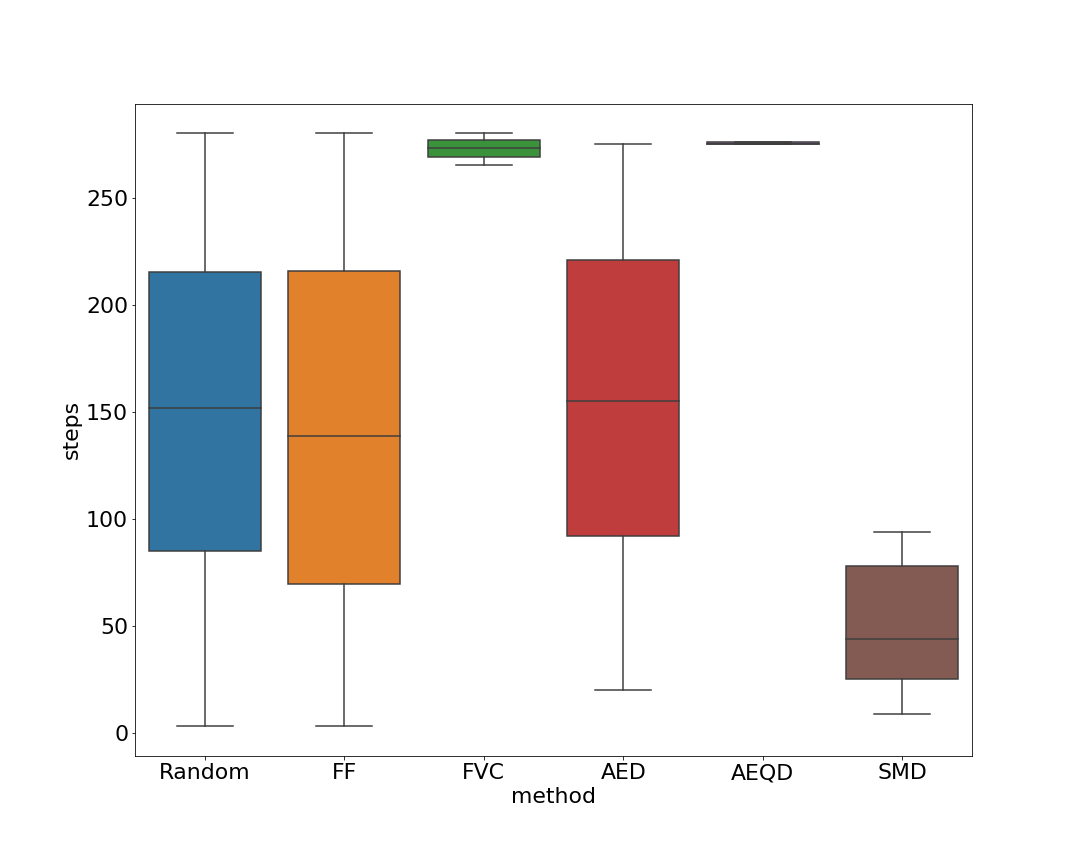
\includegraphics[width=1\linewidth, height=\linewidth]{chapters/images/xSigmoid/box.png}  
  \caption{xSigmoid}
\label{fig:xSigmoid-box}
\end{subfigure}
\begin{subfigure}{.5\textwidth}
  \centering
  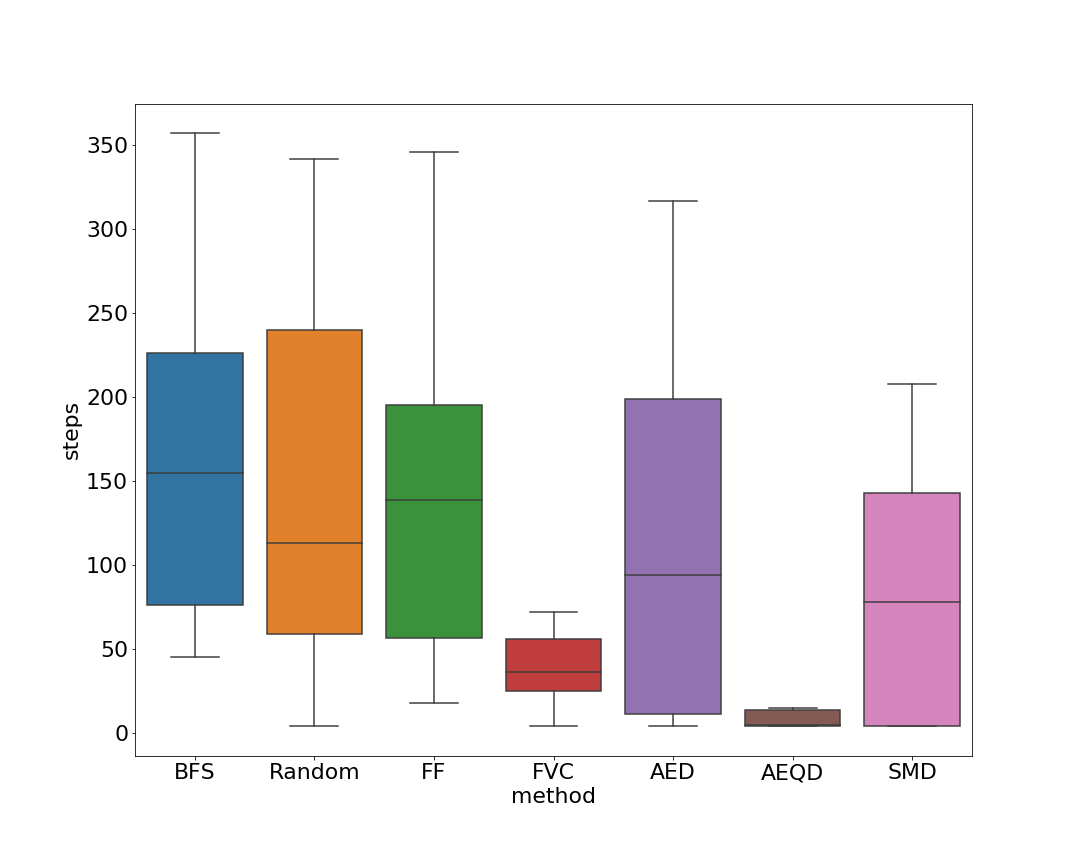
\includegraphics[width=1\linewidth, height=\linewidth]{chapters/images/RabinovichFabricant/4.png}  
  \caption{Rabinovich-Fabrikant}
  \label{fig:Rabinovich-Fabricant-box}
\end{subfigure}
\caption{Сравнение эвристик}
\label{fig:box-plots}
\end{figure}

Таким образом, наиболее успешно показали себя эвристики \textit{AEQD} и \textit{SMD}. Так же \textit{AED} и \textit{FVC} показывают, в целом, результаты лучшие, чем ID-DLS с отсутствием какой либо эвристики. 